% !TeX root = ./maltoni_niccolo_tesi.tex
% !TeX encoding = UTF-8 Unicode
% !TeX spellcheck = it_IT
% !TeX program = arara
% !TeX options = --log --verbose --language=it "%DOC%"

% arara: lualatex:      { interaction: batchmode }
% arara: frontespizio:  { interaction: batchmode, engine: lualatex }
% arara: biber
% arara: lualatex:      { interaction: batchmode }
% arara: lualatex:      { interaction: nonstopmode, synctex: yes }

\documentclass[%
  a4paper,                % formato di pagina A4
  fontsize=12pt,          % corpo del testo a 12pt
  % la dimensione 12pt automaticamente imposta \footnotesize a 10pt
  twoside,                % (oneside|twoside) documento a singola o doppia facciata,
  openright,              % (openany|openright) fa cominciare un capitolo nella successiva pagina a disposizione o sempre in una pagina destra
  % twocolumn,            % dà a LaTeX le istruzioni per comporre l'intero documento su due colonne
  titlepage,              % (titlepage|notitlepage) se dopo il titolo del documento debbaavere  inizio  una  nuova  pagina
  % fleqn,                % allinea le formule a sinistra rispetto a un margine rientrato
  % leqno,                % mette la numerazione delle formule a sinistra anziché a destra
  final                   % (draft|final) scelta tra bozza o finale, influenza il comportamento degli altri pacchetti
  headings=standardclasses, % changes the font of all section heading levels to serif
  headings=big,             % revert to default heading size that headings=standardclasses changes
  chapterprefix=false       % reverse the chapterprefix=true option that headings=standardclasses sets
]{scrbook}

\usepackage{fancyvrb}       % fornisce l'ambiente VerbatimOut e modifica listati di codice

\begin{VerbatimOut}{\jobname.xmpdata}
\Title{Progettazione di un sistema web per la simulazione di programmi aggregati}
\Author{Niccolò Maltoni}
\Copyright{Questo documento è fornito sotto licenza Creative Commons Attribution-ShareAlike 4.0 International}
\CopyrightURL{http://creativecommons.org/licenses/by-sa/4.0}
\end{VerbatimOut}

\usepackage{unibotesi}
\usepackage[automark,headsepline]{scrlayer-scrpage}
\clearpairofpagestyles{}
\cfoot[\pagemark]{\pagemark}
\lehead{\headmark}
\rohead{\headmark}
\pagestyle{scrheadings}

\begin{document}

  \frontmatter{}

  \begin{Preambolo*}
  \usepackage{fontspec}
  \defaultfontfeatures{ Scale = MatchUppercase }
  \setmainfont{libertinusserif}[
    Scale=1.0,
    Ligatures={Common, TeX},
    % Numbers={OldStyle, Proportional},
    UprightFont={*-regular},
    BoldFont={*-bold},
    ItalicFont={*-italic},
    BoldItalicFont={*-bolditalic},
    Extension=.otf
  ]
  \setsansfont{libertinussans}[
    Ligatures={Common, TeX},
    % Numbers={OldStyle, Proportional},
    UprightFont={*-regular},
    BoldFont={*-bold},
    ItalicFont={*-italic},
    % BoldItalicFont={*-bolditalic},
    Extension=.otf
  ]
  \setmonofont{libertinusmono}[
    Scale=0.95,
    UprightFont={*-regular},
    % BoldFont={*-bold},
    % ItalicFont={*-italic},
    % BoldItalicFont={*-bolditalic},
    Extension=.otf
  ]
\end{Preambolo*}
\begin{frontespizio}
  \Universita{Bologna}        % aggiunge da sé “Università degli Studi di”.
  \Istituzione{%
    Alma Mater Studiorum --- Università di Bologna \\%
    Campus di Cesena%
  }
  \Divisione{Dipartimento di Informatica --- Scienza e Ingegneria}
  \Corso[Laurea magistrale]{Ingegneria e Scienze Informatiche}
  \Annoaccademico{2019--2020}
  \Titolo{Progettazione di una piattaforma web\\per la simulazione di programmi aggregati}
  \Sottotitolo{Tesi in Pervasive Computing}
  % \Preambolo{\renewcommand{\frontsmallfont}[1]{\small}}       % non viene stampata la matricola
  % \Preambolo{\renewcommand{\frontsmallfont}[1]{\small Matr.}} % abbrevia la matricola
  \Candidato[840825]{Niccolò~Maltoni}
  \NCandidato{Presentata da}  % sostituisce la parola “Candidato”
  \Relatore{Prof.~Mirko~Viroli}
  \Correlatore{Prof.~Danilo~Pianini}
  \Piede{%                    % sostituisce la scritta “Anno Accademico” nel piede
    III sessione di laurea \\%
    Anno Accademico 2019--2020%
  }
\end{frontespizio}

% Necessario per Overleaf: compila il TeX del frontespizio subito dopo averlo generato
\IfFileExists{\jobname-frn.pdf}{}{%
\immediate\write18{lualatex \jobname-frn}}

  \clearemptydoublepage{}
\thispagestyle{empty}
\vspace*{20ex}
\begin{flushright}
    \begin{LARGE}
        \textbf{Parole chiave}\\
        \vspace{5ex}
    \end{LARGE}
    \begin{normalsize}
        \textbf{%
            Parola chiave 1\\%
            \medskip
            Parola chiave 2%
        }
    \end{normalsize}
\end{flushright}
\vfill

  % !TeX root = ../../maltoni_niccolo_tesi.tex
% !TeX encoding = UTF-8 Unicode
% !TeX spellcheck = it_IT

\clearemptydoublepage{}
\null{}\vspace{\stretch{1}}
\begin{flushright}
    \textit{Dedica}
\end{flushright}
\vspace{\stretch{2}}\null{}

  \begin{abstract}
  % \strong{TODO}
  \todo[inline]{Il sommario verrà scritto per ultimo; di seguito un lorem ipsum per dare l'idea}
  \lipsum[1-2] % ChkTeX 8
\end{abstract}


  \tableofcontents

  \mainmatter{}

  \addchap{Introduzione}

  \part{Background}
    \chapter{Motivazioni}\label{ch:motivations}

  \unsure[inline]{
    Secondo me, questo capitolo dovrebbe essere inserito DOPO aver illustrato la programmazione aggregata e le tecnologie web.

    In questo modo, si avrebbe anche meno la sensazione di ``ripetuto'' avuta da abstract -> introduzione -> motivazioni tutte in fila.
  }

  Come detto nell'\nameref{ch:intro}, il rapido aumento di dispositivi capaci di computare e distribuiti nell'ambiente ha reso necessario ideare nuovi paradigmi di programmazione.
  Uno di questi è senza dubbio l'\emph{aggregate programming}, di cui si tratterà più nel dettaglio nel~\Cref{ch:aggregate}.
  In questo \nameCref{ch:motivations}, invece, verrà analizzato lo stato dell'arte relativamente alla creazione di un programma aggregato,
  mettendo in evidenza le ragioni per la quale è stato realizzato questo progetto di tesi.

  \section{Stato dell'arte}\label{sec:state-of-art}

  Prima di partire con la progettazione del sistema, è stato necessario valutare lo stato dell'arte nel quale il software va ad inserirsi.
  % Si è dunque deciso di analizzare nel dettaglio quali sono i punti critici dello stato dell'arte;
  % i
  In particolare, si è preso in considerazione la procedura di configurazione di un progetto realizzato in un linguaggio aggregato,
  confrontandolo con l'esperienza di sviluppo ottenuta con altri linguaggi in altri contesti.

  \subsection{Iniziare un progetto Protelis}\label{subsec:setup}

  I due principali linguaggi di programmazione aggregata che implementano il modello teorico del field calculus sono Protelis e ScaFi.
  ScaFi è un DSL interno a Scala e, come tale, richiede di essere utilizzato all'interno di questo linguaggio;
  poiché sono già state realizzate tesi~\cite{amslaurea12188,amslaurea16824} incentrate sull'esecuzione di ScaFi,
  è stato richiesto di concentrarsi, in questa tesi, solamente su Protelis.

  Protelis è un linguaggio \emph{Java-hosted} e, come tale, deve essere caricato in un progetto JVM che esegue un'istanza del suo interprete.
  Di seguito sono riportate le possibili modalità di esecuzione documentate nello stato dell'arte.

  \begin{description}
    \item[Alchemist]\cite{ProtelisSAC14}
      Una prima possibilità di utilizzo è tramite il simulatore Alchemist~\cite{alchemist-jos2013}.
      Esso mette infatti a disposizione all'interno del proprio meta-modello un'incarnazione specifica per Protelis.
      Esso permette la simulazione di reti con pattern anche complessi con semplici file di configurazione.
      In~\Cref{fig:alchemis-protelis} sono riportate le entità in gioco.

      \begin{figure}[htbp]
        \centering
        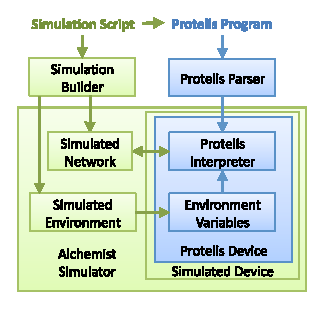
\includegraphics[width=0.52\textwidth]{res/fig/protelis-alchemist-arch.eps}%
        \caption[
          Implementazione dell'architettura di Protelis in Alchemist
        ]{
          Implementazione dell'architettura di Protelis in Alchemist.

          \nameCref{fig:alchemis-protelis} ripresa da~\cite{ProtelisSAC14}.
        }%
        \label{fig:alchemis-protelis}
      \end{figure}

      Alchemist può essere utilizzato all'interno di altro software in ambiente Java come libreria di virtualizzazione, oppure in modo indipendente tramite linea di comando\footnote{\url{https://github.com/Protelis/Protelis-Alchemist-tutorial}}.
      In questo secondo caso, è possibile definire il codice Protelis insieme a file YAML di configurazione ed utilizzare il file jar eseguibile di Alchemist.
      Il simulatore mette a disposizione un'interfaccia grafica minimale per la visualizzazione e il controllo della simulazione.

    \item[ProtelisVM]\cite{amslaurea19778}
      Un'altra possibilità, più moderna, è tramite l'importazione del framework di Protelis nel \emph{classpath} di un progetto Java, ad esempio prelevandolo come dipendenza Maven.
      Il framework mette a disposizione una classe denominata \texttt{ProtelisVM} (\Cref{fig:protelisvm}), che si occupa di eseguire un programma Protelis in un \texttt{ExecutionContext},
      ossia un'astrazione del dispositivo esecutore che si frappone tra la macchina virtuale e l'ambiente fisico.

      \begin{figure}[htbp]
        \centering
        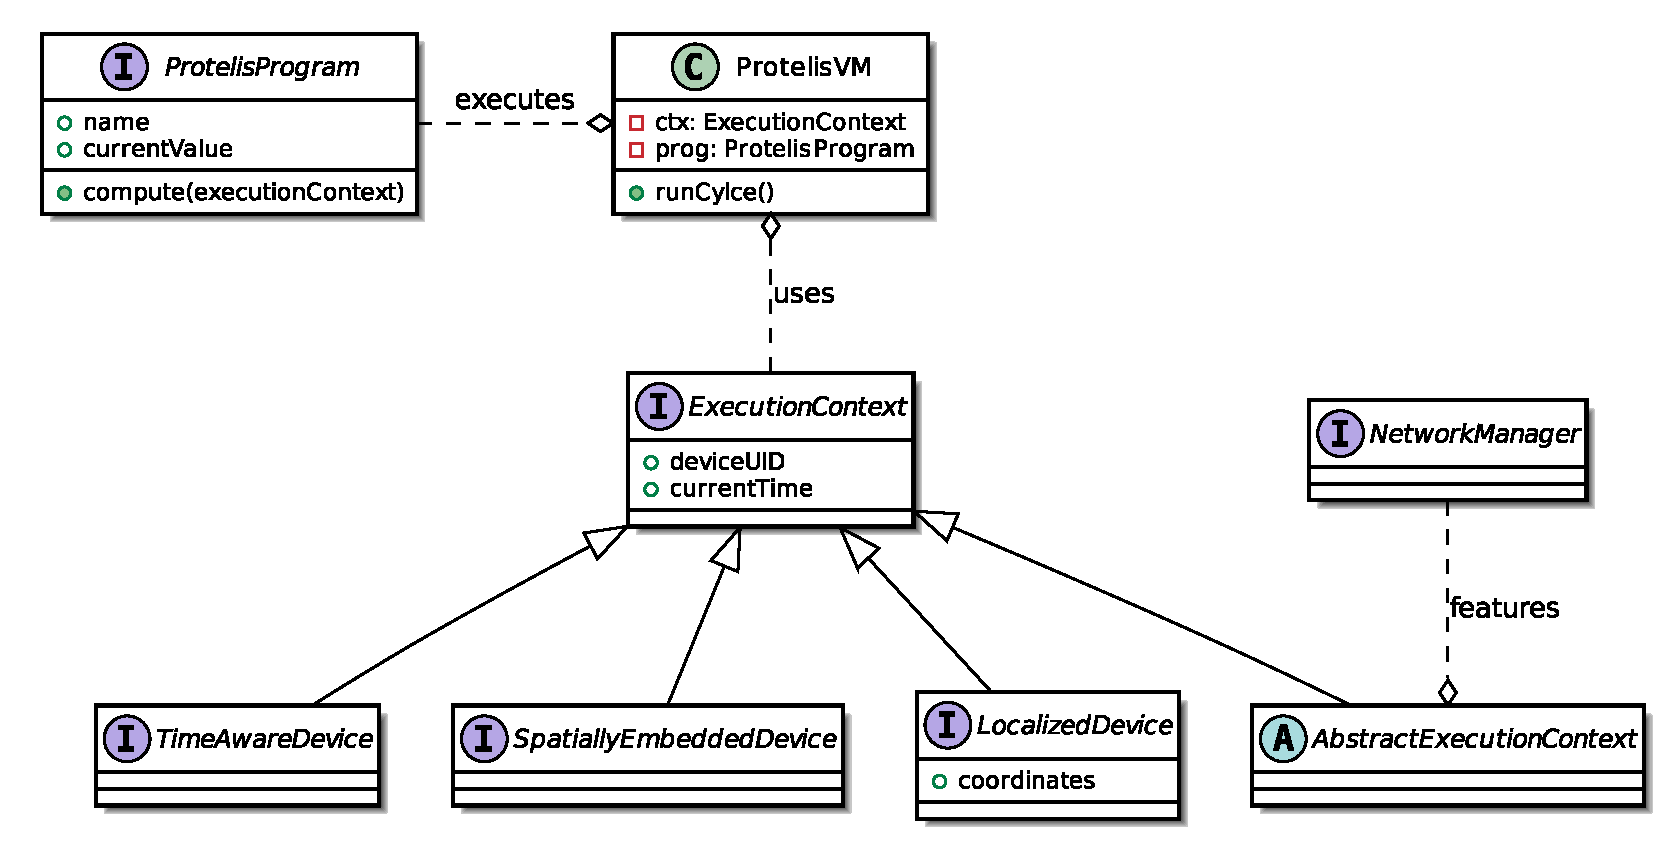
\includegraphics[width=0.87\textwidth]{res/uml/ExecutionContext.eps}%
        \caption{UML delle principali entità del framework di Protelis}%
        \label{fig:protelisvm}
      \end{figure}

      Attraverso la libreria è possibile definire dispositivi virtuali o, potenzialmente, collegare implementazioni fisiche.
      Su GitHub\footnote{\url{https://github.com/Protelis/Protelis-Demo}} sono riportati alcuni esempi con diverse opzioni di integrazione.

    \item[NASA WorldWind]\cite{4161692}
      Un'ultima possibilità vede invece l'utilizzo del framework di visualizzazione open-source WorldWind, sviluppato dalla NASA\@.
      Esso è stato utilizzato per dimostrare come Protelis possa essere uno strumento che permette di controllare anche dispositivi reali come uno sciame di droni.
      Il codice della demo è pubblico su GitHub\footnote{\url{https://github.com/Protelis/Protelis-Demo-Visualized}}.
  \end{description}

  In ciascuno di questi esempi risulta evidente che la configurazione di un progetto per Protelis, anche estremamente minimale, coinvolge strumenti esterni la cui complessità può non essere banale.
  Sarebbe interessante avere a disposizione un ambiente di sviluppo che non richieda configurazione e permetta di provare prototipi di codice durante l'apprendimento del linguaggio.

  \subsection{Ambienti di sviluppo online}\label{subsec:online-ide}

  Con il progredire delle capacità delle applicazioni JavaScript per browser e della popolarità del linguaggio stesso, sono nate numerose implementazioni di IDE (\emph{Integrated Development Environment}) in grado di eseguire all'interno di una pagina web, comunicando al più con un \emph{language server} remoto.
  Inizialmente appannaggio di ambienti per la prototipazione di codice JavaScript (in quanto si avvalevano del motore nativamente integrato nel browser per l'esecuzione), recentemente molti linguaggi offrono un ambiente, spesso chiamato \emph{playground}, in cui sperimentare (ad esempio Kotlin, TypeScript o Scala).

  Alcuni ambienti di questo tipo, addirittura, sono in grado di offrire un'esperienza utente tanto immediata e completa da venire preferiti a installazioni desktop tradizionali.
  È questo il caso, ad esempio, di Overleaf. \unsure{Dovrei inserire delle immagini descrittive (come uno screenshot)? Secondo me sono più corrette nella sezione di design, ma potrebbero starci anche qua}

  Overleaf\footnote{\url{https://www.overleaf.com}} è un editor per \LaTeX{} completamente online che permette all'utente di scrivere documenti tramite browser;
  il sorgente del markup viene compilato in modo trasparente all'utente, il quale deve preoccuparsi unicamente del contenuto che sta scrivendo.
  Questo risparmia agli utenti inesperti la fase di installazione e configurazione di una distribuzione \LaTeX{} e la scelta di un editor tra i tanti disponibili.

  Potrebbe essere interessante offrire all'utente novizio di Protelis un'esperienza simile:
  la rete di dispositivi (reale o simulata) viene configurata nel server, insieme all'interprete per il linguaggio.
  L'utente avrebbe dunque a disposizione, tramite il proprio browser, solo un semplice editor per scrivere il codice e metterlo in esecuzione.

  \section{Prospettive e approccio al problema}\label{sec:prospective}

  \unsure[inline]{
    Dovrei dire altro nella descrizione dell'approccio al problema?

    Temo di ripetermi con quello che dirò più avanti nei requisiti (e un po' nella loro analisi e nella progettazione).
  }

  Terminata la disamina dello stato dell'arte, è possibile delineare un approccio concreto al problema.
  L'intenzione è quella di realizzare un sistema software distribuito che offra all'utente la possibilità di utilizzare un linguaggio di programmazione aggregata nel modo più trasparente possibile.
  In particolare, tramite un'interfaccia Single-Page accessibile tramite browser, l'utente dovrebbe poter accedere alle API di un server che nascondono completamente tutta la complessità di configurazione di una rete (reale o simulata) e di un progetto Java/Scala.

  Il linguaggio di riferimento per il prototipo dovrebbe essere Protelis, ma il sistema dovrebbe, potenzialmente, essere estendibile a ScaFi e ad altri linguaggi futuri simili.

    \chapter{Programmazione aggregata}\label{ch:aggregate}

\unsure[inline]{
  Alcuni concetti di programmazione aggregata, come le dicevo per mail, mi hanno richiesto un po' di tempo per saperli spiegare.

  Spero di non aver capito male delle cose o essere stato impreciso.
}

La crescita esponenziale di dispositivi informatici di varia natura inseriti in contesti quotidiani ha avuto un impatto globale notevole.
Questo insieme di entità connesse (\Cref{fig:iot}) ha dato luogo a ciò che viene definito \emph{Internet of Things} (\emph{IoT}).

\begin{figure}[htbp]
  \centering
  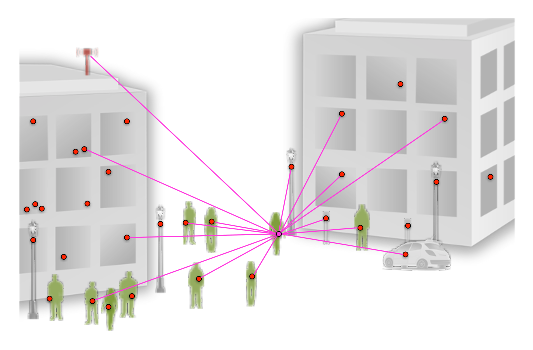
\includegraphics[width=0.8\textwidth]{res/fig/iot.eps}%
  \caption[
    Possibile scenario di rete in contesto urbano.
  ]{
    Possibile scenario di rete in contesto urbano.

    \nameCref{fig:iot} ripresa da~\cite{7274429}.
  }%
  \label{fig:iot}
\end{figure}

L'approccio tradizionale per la realizzazione di sistemi in questo contesto è sempre stato con paradigma ``\emph{single device view point}'',
in cui l'unità fondamentale è il singolo dispositivo connesso con il mondo fisico e con gli altri device, il cui insieme dei comportamenti individuali determinava il funzionamento del sistema.
Tale approccio si è rivelato inadeguato, in quanto un elevato numero di dispositivi (possibilmente eterogenei) pone diversi problemi legati all'organizzazione della rete
e la sua gestione che non dovrebbero essere gestiti in questo livello di astrazione.

L'\emph{aggregate programming}, o \emph{programmazione aggregata}, costituisce un'alternativa all'approccio ``classico''
volta a semplificare la progettazione, creazione e manutenzione di sistemi distribuiti complessi.
La programmazione aggregata, infatti, ragiona su più larga scala, cercando di spostare l'attenzione sul \emph{collettivo di dispositivi} che collaborano;
i dettagli relativi al singolo device devono essere ignorabili, per quanto possibile~\cite{7274429}.

L'idea alla base è dunque di definire una modalità di deduzione del comportamento locale al singolo dispositivo a partire dal comportamento globale, di più alto livello,
effettuando un \emph{mapping da globale a locale}.
I due punti di vista necessari per poter raggiungere un tale livello di astrazione sono due~\cite{aggregatescala-pmldc2016}:

\begin{itemize}
    \item
        il primo, detto locale o \emph{device-centric}, è quello che si riferisce alla computazione aggregata eseguita dal dispositivo singolo.
        Questa può essere considerata la vista tradizionale.
    \item
        il secondo, detto globale o \emph{aggregate view}, si riferisce invece alla computazione svolta dal sistema aggregato come singola unità.
        Rispetto all'approccio tradizionale, tale punto di vista sposta maggiormente l'attenzione dal \emph{come} il sistema possa funzionare
        al \emph{cosa} effettivamente si desidera che faccia.
\end{itemize}

In generale, le strategie principali per adottare un livello di astrazione così elevato sono state formalizzate nelle seguenti possibilità~\cite{7274429}:

% TODO: rielabora traduzione
\begin{itemize}
  \item rendere le interazioni tra i dispositivi implicite (come ad esempio nell'approccio \emph{TOTA}, ``\emph{Tuples On The Air}''~\cite{10.1145/1538942.1538945});
  \item comporre comporre costruzioni geometriche e topologiche (ad esempio, \emph{Origami Shape Language}~\cite{nagpal2001programmable});
  \item dividere la computazione in modo automatico per le esecuzioni sullo stile di modelli di \emph{computazione cloud} come \emph{MapReduce}~\cite{10.1145/1327452.1327492};
  \item sintetizzare i dati provenienti da regioni spazio-temporali e inviarli come stream ad altre regioni (ad esempio, \emph{TinyDB}~\cite{1017485});
  \item fornire costrutti generalizzabili per la computazione spazio-temporale (ad esempio, \emph{Protelis}~\cite{PianiniSASOTutorial2017}, di cui tratteremo meglio in~\Cref{sec:protelis}).
\end{itemize}

Studiando i suddetti approcci, sono state osservate le seguenti proprietà dei sistemi situati su larga scala:

% TODO: rielabora traduzione
\begin{itemize}
  \item laddove non è richiesta al programmatore alcuna interazione, i meccanismi per la coordinazione devono essere nascosti ``\emph{under the hood}''~\cite{7274429};
  \item la composizione dei moduli deve essere tanto semplice quanto trasparente;
  \item sottoinsiemi differenti necessitano di meccanismi di coordinazione differenti per regioni e tempi distinti.
\end{itemize}

Per affrontare queste problematiche, la programmazione aggregata si basa sui seguenti tre principi~\cite{7274429}:

\begin{itemize}
  \item la ``macchina'' programmata non deve essere il singolo dispositivo, bensì la \emph{regione} dell'ambiente computazionale che astrae dai dettagli specifici;
  \item il ``programma'' è specificato come \emph{manipolazione di costrutti di dati} con estensioni spaziali e temporali in tutta la regione;
  \item tali manipolazioni vengono eseguite dai dispositivi inseriti all'interno della regione, tramite l'uso di meccanismi di coordinazione resilienti e di interazioni basate sulla prossimità.
\end{itemize}

In questo modo, i meccanismi di coordinazione, spesso complessi, vengono nascosti facilitando la costruzione e favorendo la modularità.
In particolare, il paradigma si struttura su più livelli di astrazione, come è possibile vedere in~\Cref{fig:stack}.

\begin{figure}[htbp]
  \centering
  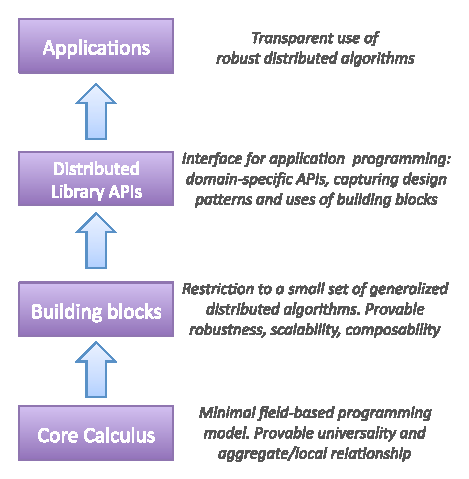
\includegraphics[width=0.6\textwidth]{res/fig/stack-2.eps}%
  \caption[
    Principali livelli dell'\emph{Aggregate Programming}.
  ]{
    Principali livelli dell'\emph{Aggregate Programming}.

    \nameCref{fig:stack} ripresa da~\cite{ProtelisSAC14}.
  }%
  \label{fig:stack}
\end{figure}

Nelle \nameCrefs{sec:field-calculus} successive analizzeremo più nel dettaglio alcuni di questi.

\section[Field calculus]{Field calculus \& Building Blocks}\label{sec:field-calculus}

Al livello più basso della struttura rappresentata in \Cref{fig:stack} si trova il \emph{field calculus}~\cite{FieldCalculusFOCLASA2013}.
Esso è un \emph{core calculus}, ovvero un modello teorico di programmazione che riassume la semantica operazionale minimale necessaria alla progettazione di un sistema aggregato.

Il field calculus si basato sul concetto di \emph{campo computazionale}~\cite{FieldCalculusFOCLASA2013}:
il termine riprende la nozione di campo in fisica~\cite{mcmullin2002origins}, esteso al concetto di computazione
e inteso come ``una proiezione di ciascun dispositivo computazionale nello spazio verso un oggetto computazionale arbitrario'',
ossia l'applicazione di una funzione che, in un dato momento nel tempo, mappa ogni punto dello spazio (un dispositivo o un nodo),
verso un oggetto computazionale (un valore) che rappresenta il risultato della computazione su quel device.
I \emph{campi} sono strutture dati distribuite a livello di aggregazione che gradualmente si adattano ai cambiamenti della topologia sottostante e alle interazioni con l'ambiente.

I campi vengono generati e manipolati attraverso cinque costrutti fondamentali~\cite{BV-FOCAS2014,computationalfields-forte2015}:

\unsure[inline]{
  Qui ho espresso gli operatori con la sintassi (mi pare di capire LISP-like, credo ripresa da Proto) che veniva utilizzata nei primi paper sull'argomento.

  Va bene? Oppure dovrei usare le notazioni che avete usato nei paper più recenti (che invece penso si appoggino alla sintassi Protelis)?
}

\begin{description}
  % TODO: should I use new notation?
  \item[Built-in operator] \((\,\texttt{b\,(e\textsubscript{1}\:\dots{}\:e\textsubscript{n})}\,)\) \\
    Un operatore \emph{built-in} \texttt{b} modella in modo uniforme operazioni basate su valori puntuali, cioè che non coinvolgono né lo stato, né la comunicazione.
    Esso determina il valore del campo in output all'evento \texttt{m} (un punto nello spazio-tempo) solo dai valori dello spazio \texttt{e}
    e dei campi in input \(\texttt{e\textsubscript{1}\:\dots{}\:e\textsubscript{n}}\).
    Possono essere funzioni \emph{stateless} matematiche, logiche o algoritmiche, ma anche sensori, attuatori, funzioni di libreria, ecc.
  % TODO: should I use new notation?
  \item[Function definition and call] \((\,\texttt{def\ f\,(x\textsubscript{1}\:\dots{}\:x\textsubscript{n})\ e}\,)\) \\
    Astrazione e ricorsione sono supportate attraverso la definizione di funzione:
    una funzione \texttt{f} con parametri formali \(\texttt{x\textsubscript{1}\:\dots{}\:x\textsubscript{n}}\) e corpo \texttt{e}
    può essere dichiarata con la sintassi \emph{Lisp-like} di cui sopra e invocata con \((\,\texttt{f\,(e\textsubscript{1}\:\dots{}\:e\textsubscript{n})}\,)\).
  % TODO: should I use new notation?
  \item[Time evolution] \((\,\texttt{rep\ x\;e\textsubscript{0}\;e}\,)\) \\
    Il costrutto di ripetizione supporta l'evoluzione dinamica dei campi, assumendo che ciascun dispositivo computi il proprio programma ripetutamente in \emph{round} asincroni.
    La variabile di stato \texttt{x} è inizializzata con il risultato della valutazione dell'espressione \texttt{e\textsubscript{0}} e aggiornato ad ogni step computando \texttt{e} in relazione al precedente valore di \texttt{x}.
  % TODO: should I use new notation?
  \item[Neighborhood values] \((\,\texttt{nbr\ e}\,)\) \\
    L'interazione diretta tra i dispositivi è incapsulata nel costrutto \texttt{nbr};
    con esso, si ottiene campo per ogni dispositivo, il quale è una mappa da tutti i vicini al loro più recente valore di \texttt{s}.
    Funzioni ``\emph{hood}'' \emph{built-in} possono poi riassumere queste mappe.
  % TODO: should I use new notation?
  \item[Domain restriction] \((\,\texttt{if\ e\textsubscript{0}\;e\textsubscript{1}\;e\textsubscript{2}}\,)\) \\
    La ramificazione distribuita è implementata dal costrutto \texttt{if}, che permette di suddividere la rete in due regioni:
    una nella quale l'espressione \texttt{e\textsubscript{0}} è vera, nel quale \texttt{e\textsubscript{1}} viene computato, e una nella quale è falsa, che invece computerà \texttt{e\textsubscript{2}}.
    Tali suddivisioni sono incapsulate e non possono avere effetti al di fuori dei relativi sottospazi.
\end{description}

Questi costrutti permettono al \emph{field calculus} di essere universale~\cite{beal2014towards}, supportando ogni computazione spazio-temporale causale e approssimabile.
Tramite questi operatori, inoltre, sono garantite:
\begin{inparaitem}
  \item \emph{portabilità},
  \item \emph{indipendenza} dall'infrastruttura,
  \item \emph{integrazione} con servizi non aggregati.
\end{inparaitem}

\unsure[inline]{
  Gli elenchi in-line a me piacciono per elenchi di singole parole, al posto di una semplice riga separata da virgole.

  So che da molti sono considerati accettabili solo per i paper con limite di lunghezza per risparmiare spazio in elenchi veri e propri, non per questo uso.
  Lei che ne pensa?
}

Per poter garantire anche \emph{resilienza} alla coordinazione, è necessario introdurre il livello di astrazione successivo:
gli operatori ``\emph{building block}''~\cite{BV-FOCAS2014}.

Questo layer consiste di un insieme di operatori generici e di più alto livello, che offrono allo sviluppatore un ambiente di programmazione più espressivo,
contribuendo in particolare alla cosiddetta \emph{self-stabilization}, ossia la capacità di raggiungere uno stato atteso in un numero finito di passi,
indipendentemente dallo stato di partenza.
Tale proprietà è garantita per tutti i campi ottenuti tramite composizione funzionale~\cite{BV-FOCAS2014}.

\begin{figure}[htbp]
  \centering
  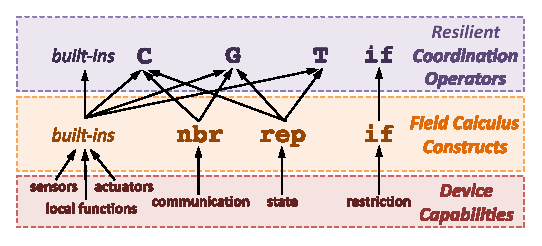
\includegraphics[width=0.8\textwidth]{res/fig/stack-detail-crop.eps}%
  \caption{Dettaglio dei livelli più bassi dell'\emph{Aggregate Programming}.}%
  \label{fig:stack-detail}
\end{figure}

Come riportato in~\Cref{fig:stack-detail}, i \emph{building block} individuati in aggiunta al costrutto \texttt{if} del \emph{field calculus} sono tre operatori di coordinazione~\cite{7274429,BV-FOCAS2014}:

\unsure[inline]{Qui mi rendo conto che le traduzioni sono brutte e verbose. Posso metterle in inglese?}

\unsure[inline]{Dovrei espandere la descrizione? Dovrei riportare il costrutto comprensivo di parametri? (con l'italiano non ci sta nella riga)}

\begin{description}
  \item[Diffusione dell'informazione nello spazio] \texttt{G} \\ % Spreading Information Across Space
    % \texttt{G(source, init, metric, accumulate)} \\ % ChkTeX 36
    Quest'operatore generalizza operazioni molto comuni come la stima della distanza e messaggi broadcast.
  \item[Raccoglimento di informazione attraverso lo spazio] \texttt{C} \\ % Collecting Information From Across Space
    % \texttt{C(potential, accumulate, local, null)} \\ % ChkTeX 36
    Quest'operatore aggrega le informazioni verso la sorgente attraverso il gradiente di un campo specificato.
  \item[Riassunto dell'informazione nel tempo] \texttt{T} \\ % Summarizing Information Across Time
    % \texttt{T(init, floor, decay)} \\ % ChkTeX 36
    Quest'operatore generalizza un timer il cui rateo di aggiornamento può variare nel tempo.
\end{description}

Questi operatori sono sufficientemente espressivi da poter coprire, da soli o combinati tra loro, tutti i pattern di coordinazione usati nei sistemi a larga scala.

Come livello di astrazione ulteriore (il secondo dall'alto nella~\Cref{fig:stack}), volto a semplificare la composizione dei \emph{building blocks}, si aggiungono le API \emph{general-purpose}~\cite{amslaurea13090}.
Esse possono essere usate e composte tra loro per scrivere applicazioni distribuite senza preoccuparsi dei meccanismi di coordinazione, la cui robustezza è garantita dagli operatori descritti sopra.

% \section[Protelis]{Protelis, Programming Language for Aggregate Computing}\label{sec:protelis}
\section{Protelis}\label{sec:protelis}

% \begin{wrapfigure}{r}{0.2\textwidth}
%   \begin{center}
%     
\includegraphics[width=0.2\textwidth]{res/fig/protelis-logo.png}%
%     \caption{Logo}%
%     \label{fig:protelis}
%   \end{center}
% \end{wrapfigure}

% \begin{wrapfigure}{r}{0pt}
%   \centering
%   % \vspace{-52pt}
%   
\includegraphics[width=0.2\textwidth]{res/fig/protelis-logo.png}
%   % \vspace{50pt}
%   \caption{Logo}%
%   \label{fig:protelis}
% \end{wrapfigure}

Field calculus è solamente un impianto teorico.
Vista la necessità di un'architettura portabile in grado di gestire gli aspetti di comunicazione, esecuzione e interfacciamento con hardware e sistema operativo, è stato realizzato Protelis.

\emph{Protelis}~\cite{PianiniSASOTutorial2017} è un linguaggio di programmazione aggregato di paradigma funzionale fortemente influenzato da Proto~\cite{Beal2006}.
Il linguaggio incorpora le principali funzionalità di computazione spaziale di field calculus in una sintassi più simile ai linguaggi strutturati tradizionali come C o Java.

\begin{figure}[htbp]
  \centering
  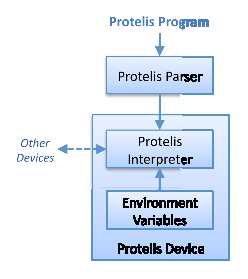
\includegraphics[width=0.4\textwidth]{res/fig/protelis-abstract-arch.eps}
  \caption[
    Architettura di Protelis
  ]{
    Architettura di Protelis.

    Figura ripresa da~\cite{ProtelisSAC14}.
  }%
  \label{fig:protelis-stack}
\end{figure}

% \begin{wrapfigure}{l}{0pt}
%   \centering
%   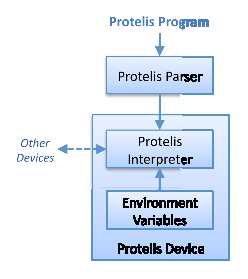
\includegraphics[width=0.4\textwidth]{res/fig/protelis-abstract-arch.eps}
%   \caption{Architettura di Protelis}%
%   \label{fig:protelis-stack}
% \end{wrapfigure}

Un nodo Protelis è costituito da un parser che traduce il programma in codice eseguibile, il quale è poi eseguito a intervalli regolari da un interprete, che si fa carico degli aspetti di interazione con il vicinato e con l'ambiente.
Ogni esecuzione è chiamata \emph{computational round}.

Il linguaggio e l'interprete sono basati su Java e possono essere inseriti in contesti virtuali~\cite{ProtelisSAC14} o reali indifferentemente.
Questo offre, da un lato, la portabilità e il supporto alle differenti piattaforme che la JVM (\emph{Java Virtual Machine}) mette a disposizione, dall'altro l'estendibilità che l'ecosistema di librerie Java può offrire.

Nel mondo scientifico, il linguaggio è già stato utilizzato per la realizzazione di diversi algoritmi aggregati.
Di seguito sono riportati alcuni esempi.

% \begin{itemize}
%   \item \emph{rendezvous} durante un evento di massa~\cite{ProtelisSAC14};
%   \item gestione di reti di servizi~\cite{7306601};
%   \item integrazione con servizi di realtà aumentata~\cite{PCRV-SCOPES2015}.
% \end{itemize}

\begin{description}
  % \item[Rendezvous durante un evento di massa]\cite{ProtelisSAC14}
  %   % Un problema tipico degli eventi di massa è la possibilità di due individui di incontrarsi in un determinato punto, in quanto la presenza elevata di dispositivi complica l'accesso a servizi cloud.
  %   Tramite Protelis, è stato possibile definire un algoritmo che consente a due persone che partecipano ad un evento di massa di incontrarsi in un punto intermedio, evitando le zone ad alta densità.

  % \item[Stima di pericolosità di una zona]\cite{BV-FOCAS2014}
  %   Basandosi sulla densità dei dispositivi in una zona, è stato possibile stimarne la pericolosità e definire modalità di dispersione efficaci.

  % \item[Algoritmi legati all'affollamento]
  %   Un problema tipico degli eventi di massa è la possibilità di due individui di incontrarsi in un determinato punto.
  %   Tramite Protelis, è stato possibile definire un algoritmo di \emph{rendezvous}~\cite{ProtelisSAC14} in grado di evitare le zone ad alta densità.

  %   In un altro progetto, basandosi sulla densità dei dispositivi in una zona, è stato possibile stimarne la pericolosità e definire modalità di dispersione efficaci.

  \item[Algoritmi legati all'affollamento]
    Tramite Protelis, è stato possibile~\cite{BV-FOCAS2014} stimarne la pericolosità di una data zona nell'ambiente basandosi sulla densità dei dispositivi presenti e definire modalità di dispersione efficaci.

    In un altro progetto~\cite{ProtelisSAC14}, è stata definito un algoritmo di \emph{rendezvous} in grado di evitare le zone ad alta densità nel contesto di un evento di massa, permettendo l'incontro di due individui in un punto intermedio.

  \item[Gestione di reti di servizi]\cite{7306601}
    Un altro utilizzo significativo è stato per la realizzazione di un sistema di gestione tra servizi in rete.
    Tali servizi, talvolta datati, possono avere molte dipendenze tra loro e scarse capacità di coordinazione.
    Per evitare stati di inconsistenza, spesso l'ordine di arresto dei server è strettamente legato alle dipendenze e rende difficile l'automazione.

    Utilizzando Protelis è stato possibile realizzare un sistema in grado di organizzarsi per riavviare lo stack.
    In particolare, sono state definite entità chiamate \emph{daemon} che monitorano ciascuna uno specifico servizio e comunicano con le altre al fine di garantire l'ordine necessario.

  \item[Integrazione con servizi di realtà aumentata]\cite{PCRV-SCOPES2015}
    La programmazione aggregata è stata testata anche nell'ambito dell'AR (\emph{Augmented Reality}).

    % In particolare, è stato introdotto il concetto di \emph{campo aumentato} che combina i campi computazionali con le capacità dell'AR\@.
    Ad esempio, è possibile utilizzare visori di realtà aumentata per visualizzare nell'ambiente i campi computazionali
    o, viceversa, modellare i dati raccolti da sensori AR come campi (detti \emph{augmented fields}).
\end{description}

\unsure[inline]{Dovrei aggiungere altri dettagli su Protelis?}

% \section[ScaFi]{ScaFi, Aggregate Programming Toolkit}\label{sec:scafi}
\section{ScaFi}\label{sec:scafi}

Una tecnologia analoga è rappresentata da \emph{ScaFi} (\emph{\emph{Sca}la with computational \emph{Fi}elds})~\cite{aggregatescala-pmldc2016}:
si tratta di un framework in Scala per la realizzazione di programmi aggregati attraverso un set compatto di primitive, presentato come implementazione del field calculus alternativa a Protelis.
% Nonostante sia dunque un DSL di Scala, è sufficientemente completo da poter essere considerato un linguaggio di programmazione aggregata a sé stante.

Il framework è composto principalmente da due parti:

% \begin{itemize}
%   \item una piattaforma distribuita che permette la configurazione e l'esecuzione di sistemi aggregati.
%   \item un \emph{internal DSL} (\emph{Domain Specific Language}) di Scala che fornisce la sintassi e la semantica per i costrutti base del field calculus.
% \end{itemize}

\begin{description}
  \item[Aggregate programming support]
    La seconda parte è un \emph{internal DSL} (\emph{Domain Specific Language}) di Scala che fornisce la sintassi e la semantica per i costrutti base del field calculus.

  \item[Aggregate platform support]
    La prima parte è una piattaforma distribuita basata sul modello ad attori di Akka che permette la configurazione e l'esecuzione di sistemi aggregati.
    Essa può essere utilizzata in modalità decentralizzata (\emph{peer-to-peer} %, \Cref{fig:scafi:p2p}
    ) o in modalità centralizzata (\emph{server-based}%, \Cref{fig:scafi:server-based}
    ).

    % \begin{figure}[htbp]
    %   \centering
    %   \begin{subfigure}{0.35\textwidth}
    %     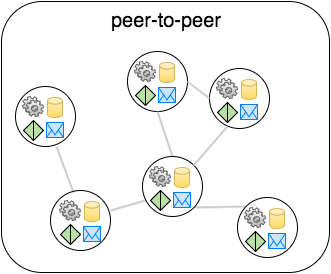
\includegraphics[width=\textwidth]{res/fig/scafi-p2p.png}
    %     \caption{Architettura \emph{peer-to-peer}}%
    %     \label{fig:scafi:p2p}
    %   \end{subfigure}
    %   \hspace{0.15\textwidth} % a differenza di \hfill il commento serve per non aggiungere spazi
    %   \begin{subfigure}{0.35\textwidth}
    %     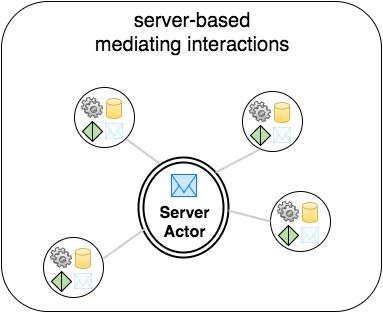
\includegraphics[width=\textwidth]{res/fig/scafi-server-based.png}
    %     \caption{Architettura \emph{server-based}}%
    %     \label{fig:scafi:server-based}
    %   \end{subfigure}
    %   \caption[
    %     Architetture della piattaforma distribuita di ScaFi
    %   ]{
    %     Architetture della piattaforma distribuita di ScaFi.

    %     Figura ripresa da~\cite{AggregatecomputingVlsubicomp16}.
    %   }%
    %   \label{fig:scafi}
    % \end{figure}

    Nel caso centralizzato, la piattaforma mantiene le posizione spaziali dei dispositivi e gestisce il vicinato, secondo il modello tradizionale client-server.
\end{description}

Basandosi su Scala come linguaggio ospite, è in grado di interoperare con Java e gli altri linguaggi in grado si eseguire in ambiente JVM, mantenendo il solido \emph{type-system} messo a disposizione da Scala e i suoi costrutti funzionali.

\unsure[inline]{Dovrei aggiungere altri dettagli su Scafi?}

    \chapter{Progettazione di sistemi web}\label{ch:web}
  Il World Wide Web ha assunto un ruolo sempre più centrale nella quotidianità delle persone e nelle dinamiche di business.
  In particolare, il modello di comunicazione è sempre più virato verso scenari distribuiti,
  nei quali piattaforme eterogenee riescono a comunicare tra loro condividendo informazioni di diverso tipo attraverso la rete internet.

  Anche i pattern di progettazione e le tecnologie implementative sono cresciute altrettanto velocemente negli ultimi anni, cambiando anche radicalmente gli approcci di interazione possibili.
  Risulta dunque importante prestare attenzione allo stato dell'arte in tal senso, chiarendo quali siano i pattern più adatti e moderni per il contesto d'uso di questa tesi.

  \section{Architetture \& paradigmi}\label{sec:web-architecture}

  Con \emph{sistema web} si intende genericamente un sistema software distribuito che coinvolge una o più entità server che espongono in rete API di varia natura, con le quali entità client possono comunicare per usufruire dei servizi.
  Generalmente, in contesto web i client sono costituiti da pagine web aperte nei browser degli utenti.

  Le possibilità di progettazione di un'applicazione web possono essere molto differenti e nel tempo si è vista una vera e propria evoluzione in tal senso.

  % \begin{enumerate}
  %   \item
  %     Nel periodo iniziale del web, ciascuna pagina web era inviata al client come un documento statico;
  %     l'interazione dell'utente con il sistema avveniva attraverso la navigazione, che comportava l'apertura di una sequenza di pagine a seconda delle esigenze.
  %     Questo tipo di interazione era però lenta, in quanto coinvolgeva sempre la ricezione di una nuova pagina dal server.
  %   \item
  %     Successivamente, nel 1995, con l'introduzione da parte di NetScape di JavaScript (di cui tratteremo meglio nella~\Cref{subsec:js}) come linguaggio di scripting client-side, i programmatori hanno avuto la possibilità di inserire elementi dinamici nelle pagine web.
  %     In questo modo, era possibile effettuare alcune operazioni anche localmente, riducendo di fatto il numero di pagine intere scambiate con il server.
  %   \item
  %     Un'ulteriore innovazione apparve l'anno seguente, quando Macromedia introdusse \emph{Flash}:
  %     esso era un plugin per i browser che permetteva di riprodurre animazioni vettoriali e gestire le interazioni con l'utente, in modo simile a quanto fatto da JavaScript.
  %   \item
  %     Il termine ``\emph{web application}'' nasce però con l'introduzione della versione 2.2 della Java Servlet Specification~\cite{java1999specification} nel 1999.
  %     anche in questo caso, però, il server ha un ruolo centrale e ancora il concetto di \emph{ajax} (\emph{Asynchronous JavaScript + XML}) non è stato introdotto.
  %   \item
  %     Successivamente vi sono stati diversi miglioramenti incrementali, fino ad arrivare allo standard HTML5~\cite{Smith2008}:
  %     quest'ultimo, infatti, introduce il supporto nativo ai contenuti multimediali ed arricchisce la semantica del documento, oltre a migliorare l'integrazione con JS\@.
  %     Con questo standard, diventa sempre più comune il concetto di \emph{Single-page application} (SPA), secondo il quale la pagina viene caricata una sola volta, e poi modificata dinamicamente tramite chiamate specifiche al server.
  %     Nascono numerosi framework client-side (come Angular, Ember o React) e l'impiego del server viene sempre più circoscritto al fornire API per accesso controllato ai dati (ad esempio, un database) o per computazioni complesse.
  % \end{enumerate}

  Nel periodo iniziale del web ciascuna pagina era inviata al client come documento statico;
  in questo caso, i server si occupavano della computazione di quanto richiesto dall'utente (anche appoggiandosi a servizi esterni tramite \emph{Common Gateway Interface}~\cite{Coar2004}) e della composizione del documento.

  Nel corso degli anni, sono stati sviluppati linguaggi di scripting (come JavaScript e Macromedia Flash) in grado di aumentare le possibilità di interazione lato client, riducendo la quantità di dati trasferiti tra il server web e il browser:
  non viene infatti più scaricata una nuova pagina ad ogni azione dell'utente, bensì solo i dati richiesti tramite chiamate \emph{ajax} (\emph{Asynchronous JavaScript And XML});
  il documento viene poi manipolato inserendo i dati ricevuti.

  Con l'avvento di HTML5~\cite{Smith2008}, viene introdotto il supporto nativo ai contenuti multimediali ed arricchita la semantica del documento;
  inoltre JavaScript riceve un supporto di prima classe e la necessità di plugin esterni come Flash diminuisce.

  Vengono sviluppati numerosi framework per la realizzazione di applicazioni costituite da una singola pagina (\emph{SPA}, \emph{Single-Page Application}), in grado di offrire l'esperienza d'uso di un applicativo desktop.
  Un applicazione web moderna normalmente è di questo tipo.

  \improvement[inline]{Dovrei aggiungere qualche immagine per ridurre l'effetto wall-of-text?}

  \improvement[inline]{
    Inizialmente avevo inserito una storia dell'evoluzione delle architetture client-side e server-side, ma poi mi sono reso conto che risultava un po' fuori contesto e l'ho tolta.

    Ritenete invece che potesse avere il suo senso come background? Nel caso posso reintegrarla velocemente.
  }

  % % Se inizialmente il server web si occupava dell'intero processo di costruzione della pagina, un po' alla volta le operazioni da effettuare per l'invio si sono sempre più ridotte.

  % % \begin{figure}[htbp]
  % %   \centering
  % %   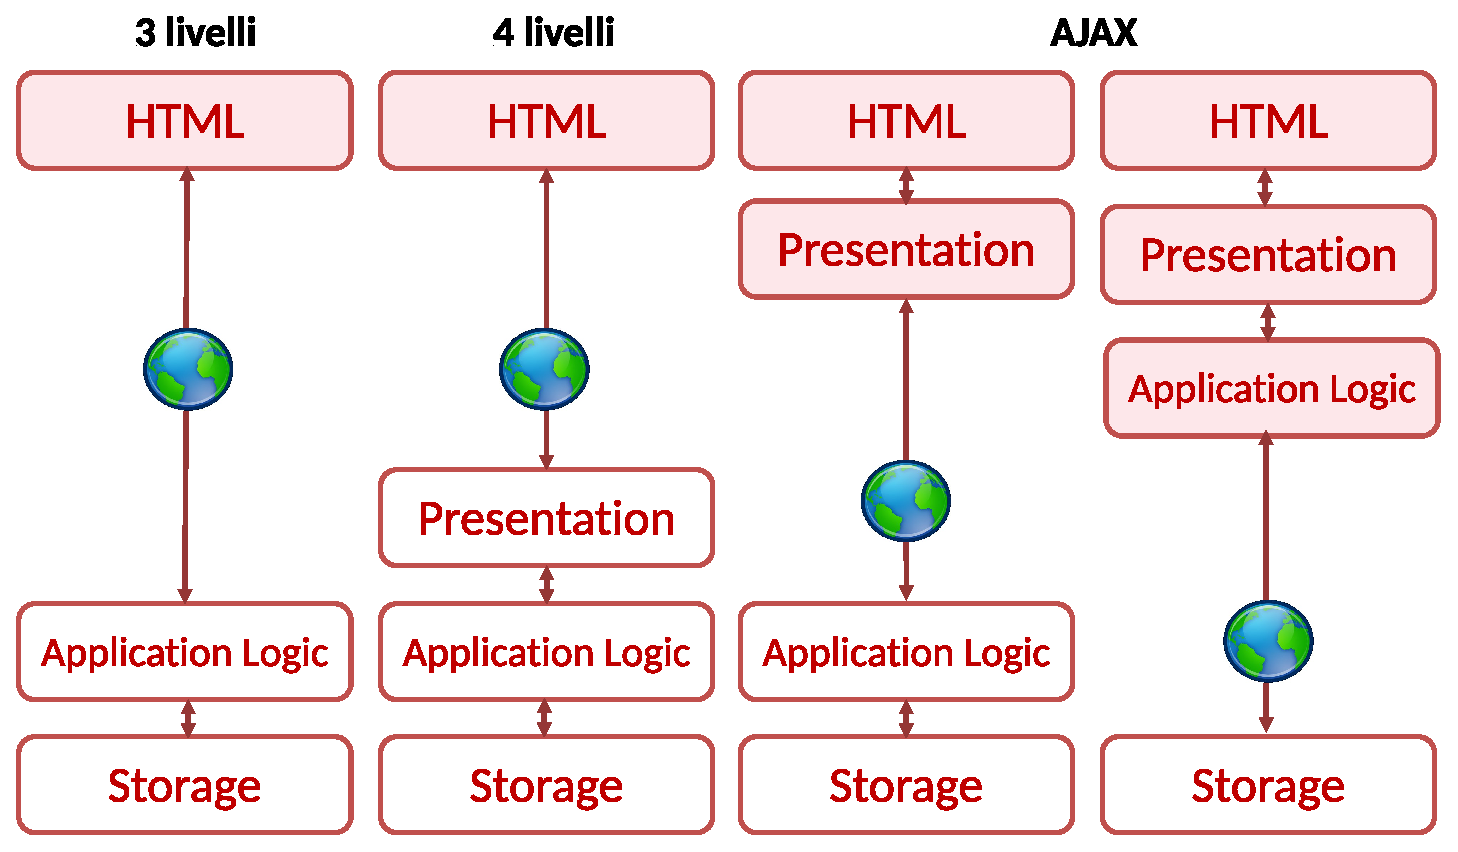
\includegraphics[width=.8\textwidth]{res/fig/server-evolution.eps}
  % %   \caption{Il controllo sulla costruzione della pagina si è spostato sempre più verso il client}%
  % %   \label{fig:server-evolution}
  % % \end{figure}

  % % In applicazioni l server diventa sempre più dedicato al memorizzare i dati (tramite database, ad esempio) e il codice client, mentre il browser si occupa di buona parte della logica applicativa.
  % Il primo approccio alla gestione della logica applicativa via rete fu quello di demandare la generazione dei contenuti a processi esterni tramite l'interfaccia standard CGI (\emph{Common Gateway Interface}~\cite{Coar2004}).
  % Essa permetteva al web server di lanciare un processo per ogni richiesta, passando i parametri necessari per l'elaborazione e di ricevere il risultato.
  % L'approccio era però poco scalabile e molto pesante per le risorse.

  \section{Linguaggi ad uso web}\label{sec:lang}
    In questa \nameCref{sec:lang} verranno analizzati i principali linguaggi di programmazione utilizzati recentemente per lo sviluppo della componente frontend delle applicazioni web.
    In particolare, verranno presi in considerazione i due linguaggi più popolari, ossia \emph{JavaScript} e il suo super-set \emph{TypeScript}, e due linguaggi di nicchia che offrono una valida alternativa: \emph{Scala.js} e \emph{Kotlin/JS}\@.

    \subsection{JavaScript e ECMAScript}\label{subsec:js}

      % \begin{wrapfigure}{r}{0pt}
      %   \centering
      %   % \vspace{-52pt}
      %   
\includegraphics[width=0.2\textwidth]{res/fig/js-logo.eps}
      %   % \vspace{50pt}
      %   \caption{Logo}%
      %   \label{fig:js}
      % \end{wrapfigure}

      \emph{JavaScript} è un linguaggio di scripting debolmente tipizzato multi-paradigma, con supporto agli stili di programmazione funzionale, ad eventi, orientato agli oggetti.
      % \begin{inparaitem}
      %   \item funzionale,
      %   \item ad eventi,
      %   \item orientato agli oggetti.
      % \end{inparaitem}
      Sviluppato originariamente nel 1995 da Brendan Eich della Netscape Communications (inizialmente con il nome di \emph{Mocha} e poi \emph{LiveScript}),
      esso è stato concepito con lo scopo di avere un linguaggio di scripting per il browser Netscape Navigator più semplice da apprendere rispetto a quelli esistenti.
      JavaScript è stato standardizzato per la prima volta nel 1997 dalla ECMA con il nome di \emph{ECMAScript}~\cite{ECMA-262,ISO:1998} e l'attuale versione è la decima.

      Il linguaggio è attualmente il più popolare per uso web, in quanto l'unico ad essere supportato da tutti i browser moderni, almeno nelle sue feature principali.
      Diversi linguaggi, come quelli che vedremo in seguito, vengono transcompilati in una versione sufficientemente supportata di JS per poter essere eseguiti nei browser.

      Analizzato dal punto di vista tecnico, esso presenta i seguenti aspetti strutturali:

      \begin{description}
        \item[Imperativo e strutturato]
          Il linguaggio si presenta con una sintassi di programmazione strutturata standard, con il supporto a tutte le strutture di controllo tradizionali.
          Una parziale differenza era nella gestione della visibilità delle variabili (\emph{scope}):
          inizialmente, JavaScript garantiva solo la visibilità a livello di funzione (\emph{function scope}) tramite la parola chiave \texttt{var};
          con ECMAScript 6 è stato aggiunto il supporto alla visibilità a livello di blocco (\emph{block scope}).

        \item[Tipizzazione dinamica]
          % https://developer.mozilla.org/en-US/docs/Web/JavaScript/Data_structures
          JavaScript è un linguaggio debolmente tipizzato:
          alle variabili non sono associati dei tipi di dato, ma solo dei valori, che possono dinamicamente cambiare tipo durante il ciclo di vita della variabile.
          La tipizzazione dinamica consente lo stile di tipizzazione chiamato \emph{duck typing}~\cite{10.1145/2103621.2103686} (o \emph{structural subtyping}):
          è possibile determinare la semantica di un oggetto in base ai metodi ed alle proprietà che esso possiede,  non in base al suo tipo.

        \item[Orientamento agli oggetti Prototype-based]
          A differenza di altri linguaggi orientato agli oggetti (come Java o C++), JavaScript non fornisce un'implementazione del concetto di \emph{classe}~\cite{Ungar1991}:
          la stessa keyword \texttt{class}, introdotta con ES6, non è altro che zucchero sintattico per migliorare l'interazione da parte dei nuovi sviluppatori con il prototipo.

          In termini di ereditarietà, infatti, JS prevede un solo costrutto: gli \emph{oggetti}.
          Ogni oggetto ha un collegamento interno ad un altro oggetto chiamato \emph{prototype}.
          Questo oggetto prototipo ha a sua volta un suo prototype, e così via finché si raggiunge un oggetto con la proprietà prototipo settata a \texttt{null}.
          \texttt{null}, per definizione, non ha un prototype ed agisce come link finale nella \emph{catena di prototipi}.

          Quasi tutti gli oggetti in JavaScript sono istanze di \texttt{Object}, che risiede in cima alla catena dei prototipi.
          % In JavaScript, è possibile aggiungere proprietà a qualsiasi oggetto in fase di esecuzione.

        \item[First-class function]
          JavaScript offre un supporto di prima classe alle funzioni, che sono considerate oggetti;
          come tali, esse possono avere delle proprietà, come ad esempio \texttt{.bind()} e \texttt{.call()}. % ChkTeX 36

          Ciascuna funzione costituisce una chiusura lessicale.

          All'interno di oggetti, proprietà di tipo funzione vengono utilizzate come costruttori e come metodi.
          Infine, le funzioni possono essere utilizzati per l'implementazione di \emph{pattern di ruolo} come i \emph{tratti} e i \emph{mixin}.

        \item[Web APIs]
          Con ECMAScript si standardizza la componente \emph{core} del linguaggio, che può eseguire in ambienti browser come su interpreti non legati strettamente al web (come ad esempio Node.js~\cite{5617064}).
          Ciascuno degli ambienti nei quali il linguaggio viene interpretato mettono a disposizione delle API specifiche per l'interazione con la piattaforma;
          quando si fa riferimento al browser, tali supporti sono chiamati \emph{Web APIs}.

          Attraverso di esse, lo sviluppatore può avere accesso agli elementi del DOM (Document Object Model) di HTML, potendo manipolare la pagina visualizzata e reagire ad eventi su di essa.

        \item[Asincronismo]
          JavaScript supporta inoltre nativamente l'esecuzione di operazioni in modo asincrono tramite il costrutto della \emph{promise}, implementato da un oggetto built-in \texttt{Promise},
          che costituisce un \emph{proxy} per un valore non necessariamente noto quando la promise viene creata.
          È poi possibile gestire il valore ottenuto con costrutti ``\emph{thenable}'' o con il \emph{pattern async/await}.
      \end{description}

    \subsection{TypeScript}\label{subsec:ts}
      TypeScript è un linguaggio di programmazione open-source sviluppato da Microsoft.
      Esso è un super-set sintatticamente rigoroso di JavaScript ES6, che si pone come obiettivi principali:

      \begin{itemize}
        \item
          l'introduzione di funzionalità \emph{cutting-edge} (talvolta anche nei primi stage di approvazione) di ECMAScript.
          Esse sono rese disponibili transcompilando il sorgente TypeScript in codice JavaScript meno recentemente ma completamente compatibile con l'ambiente di esecuzione scelto
          (ad esempio ES5 per i browser), spesso avvalendosi di \emph{polyfill} per estendere la compatibilità.
          Tra queste funzionalità, ci sono ad esempio:
          \begin{description}
            \item[Decoratori]
              Definiti in una proposta ECMAScript~\cite{decorators} tutt'ora pendente (stage 2 al momento della scrittura),
              i decoratori sono dichiarazioni (definite tramite carattere ``\texttt{@}'') associate a una dichiarazione di classe, un metodo, una proprietà o un parametro che permettono la valutazione a runtime di una espressione specificata.
              Il framework Angular, ad esempio, utilizza estensivamente questa funzionalità per effettuare \emph{dependency injection}.

            \item[Operatore di coalescenza del null \& safe navigation]
              In JavaScript, sono considerati \emph{falsy} valori come \texttt{NaN}, \texttt{0} e la stringa vuota che, pur non essendo \texttt{null} o \texttt{undefined},
              vengono trattati come valori ``non presenti'' e dunque come \texttt{false} dagli operatori booleani.
              Per ridurre la possibilità di bug dovuto a questo tipo di valori, sono stati definiti gli operatori di \emph{nullish coalescing} ``\texttt{??}'' e di \emph{safe navigation} ``\texttt{.?}''.
              Definiti sulla base di una precedente proposta ECMAScript~\cite{optional}, solo più tardi integrata, sono stati introdotti con la versione 3.7.3 di TypeScript.
          \end{description}
        \item
          l'introduzione di un sistema di tipizzazione statica opzionale che possa integrarsi nel modo più trasparente possibile nella sintassi JavaScript standard;
          in particolare, viene data la possibilità di definire tipi complessi tramite \emph{sintassi postfissa}.
      \end{itemize}

      % Di fatto, dunque, presenta tutte le caratteristiche di JavaScript descritte nella \Vref{subsec:js}.
      Il sistema di tipi viene presentato come \emph{class-based} (in contrapposizione al \emph{prototype-based} tipico di JavaScript, soprattutto prima dell'introduzione dello zucchero sintattico per le classi), ma mantiene le caratteristiche di structural subtyping citate precedentemente.
      Avvalendosi di ciò, il linguaggio permette la definizione di tipi complessi;
      è garantito il supporto ai generici, esteso da un algebra dei tipi molto flessibile che permette unione, intersezione e condizionalità, oltre alla possibilità di accesso ai tipi delle singole proprietà.

      % Il linguaggio permette la definizione di interfacce che descrivono la struttura delle proprietà attese al compilatore.
      % Tali interfacce offrono la possibilità di definire tipi complessi:

      % \begin{description}
      %   \item[Tipi funzione]
      %     Tramite le interfacce è possibile definire le strutture di funzioni, che possono essere implementate in modo anonimo nel codice attraverso il costrutto \texttt{function} o ``\emph{fat arrow}'' (\texttt{=>}).
      %     % \inputminted{typescript}{res/code/functionType.ts}
      %   \item[Indexable Types]
      %     È possibile
      % \end{description}

      % \begin{itemize}
      %   \item \emph{tipi funzione}, che definiscono l'oggetto come una funzione di una determinata struttura;
      %   \item \emph{tipi indicizzabili}, che definiscono oggetti che possono fornire l'accesso a proprietà interne tramite \emph{bracket notation} (ad esempio, l'\texttt{Array});
      %   \item \emph{tipi ibridi}, con i quali è possibile interagire tramite differenti notazioni
      % \end{itemize}

      La generazione dei metadati per la descrizione dei tipi permette un'integrazione migliore di TypeScript e JavaScript con gli ambienti di sviluppo;
      inoltre, negli anni è diventato lo standard de-facto per la documentazione dei moduli per il linguaggio sostituendo le soluzioni basate sul parsing dei commenti come JSDoc.

    \subsection{Scala.js}\label{subsec:scalajs}
      Scala.js è un compilatore per il linguaggio di programmazione Scala che genera codice JavaScript invece di bytecode per la JVM\@.
      % Questo permette l'impiego di tutte le funzionalità di Scala in contesto web, massimizzando il riuso di codice condiviso con la componente backend potenzialmente scritto con il medesimo linguaggio e in esecuzione su JVM\@.

      I principali vantaggi dell'impiego di un linguaggio come Scala all'interno del contesto web sono i seguenti:
      \begin{description}
        \item[Struttura più solida]
          Come detto, JavaScript è un linguaggio debolmente tipizzato;
          se questo aggiunge notevole flessibilità durante lo sviluppo, d'altro canto aggiunge una maggiore possibilità di bug.
          Anche TypeScript, che offre un sistema di tipi molto più completo, risulta anomalo per via della natura strutturale della tipizzazione implementata.

          Scala mette a disposizione un type system allo stesso tempo più espressivo e più rigoroso, di conseguenza può risultare più \emph{user-friendly} sia durante lo sviluppo che in fase di debug.

        \item[Prestazioni]
          Secondo benchmark~\cite{Doeraene:256862} realizzati tramite una suite estensiva già utilizzata in letteratura~\cite{10.1145/3093334.2989232}, per quanto Scala.js risulti più lento della controparte JVM, riesce ad essere fino al 33\% più veloce della controparte scritta in JavaScript.

          Inoltre, il compilatore risulta molto efficiente in termini di dimensioni finali del \emph{bundle}:
          secondo il sito ufficiale, generalmente si parte dai \(\SI{45}{\kilo\byte}\) per un'intera applicazione compressa in gzip.
          Questo permette di avere buone performance al primo caricamento dell'applicazione web.

        % \item[Interoperabilità \& riuso]
        \item[Interoperabilità con JavaScript]
          % Un terzo vantaggio risiede nelle possibilità di interoperare con codice già esistente, sia con JavaScript che con Scala.
          % In particolare,
          Scala.js è dichiaratamente compatibile con qualsiasi modulo JavaScript, purché sia dotato del codice \emph{façade} necessario per garantirne il type checking.
          Il team che mantiene il progetto ha effettuato il wrapping di numerose librerie di uso comune (50 al momento della scrittura) e mette a disposizione uno strumento di conversione automatico per le definizioni di tipo generate dal compilatore di TypeScript.
          Data la popolarità di quest'ultimo, la copertura può essere dunque considerata elevata.

        \item[Riuso]
          Un'altra compatibilità utile nella realizzazione di sistemi web di grandi dimensioni è quella con codice Scala impiegato anche nel backend.
          Questo permette di riutilizzare il codice condiviso tra server e client,
          riducendo i costi di manutenzione del medesimo codice in linguaggi differenti e la possibile \emph{friction} originata dall'etereogeneità dei linguaggi.

          Non è possibile riutilizzare codice che dipende strettamente da funzionalità della JVM (\emph{reflection}, eccezioni native di Java), in quanto porta a comportamenti indefiniti.
      \end{description}

      % Oltre al supporto semi-ufficiale a React e altri framework e librerie per la realizzazione di SPA, Scala offre un'integrazione di prima classe anche con tecnologie backend molto famose come il Play Framework di Lightbend.
      Scala inoltre ha un'integrazione molto buona con ambienti di sviluppo comunemente utilizzati, che può portare a una rilevazione degli errori più veloce e ad un autocompletamento più preciso.

    \subsection{Kotlin/Multiplatform e Kotlin/JS}\label{subsec:kotlinjs}
      Con il rilascio della versione 1.1 di Kotlin nel 2017, JetBrains ha annunciato Koltin/JS~\cite{Belov2017}, un target del compilatore in grado di generare codice JavaScript ES5 invece che bytecode per la JVM, in modo simile a quanto fatto da Scala.js.
      Il progetto si colloca in un progetto di più ampio respiro, ossia Kotlin/Multiplatform~\cite{Jemerov2017}, presentato al termine dello stesso anno in concomitanza con Kotlin 1.2, che mira a integrare anche il supporto a LLVM\@.

      L'intento è molto simile a quello di Scala.js:
      fornire un linguaggio solido per la realizzazione di componenti web (ad esempio un frontend) con lo stesso codice in esecuzione sul server su cui dialogare, in modo da coprire l'intero sistema nel modo più omogeneo possibile.

      Kotlin, a differenza di quanto avviene in Scala.js, però, prevede l'utilizzo di sorgenti differenti per la parte comune (\emph{common source set}), che modella il sistema in Kotlin puro, e per la parte specifica di un particolare target:
      in questo modo, differenti piattaforme possono avere implementazioni più vicine alle rispettive native, avvalendosi di librerie specifiche fornite dal sistema o da terze parti.
      % Questo pattern è realizzato attraverso le parole chiave \texttt{expected} e \texttt{actual} anteposte alle definizioni che

      Anche in questo caso, le criticità sono simili a quelle citate nella \nameCref{subsec:scalajs} precedente:
      \begin{itemize}
        \item
          per quanto l'intera libreria standard sia stata portata da JetBrains sulle diverse piattaforme nel modo più trasparente possibile, le piattaforme di esecuzione rimangono differenti.
          Di conseguenza, alcuni costrutti molto specifici strettamente legati alla JVM come la reflection non sono disponibili sul target JS\@.
        \item
          per garantire il supporto corretto ai tipi, è necessaria la presenza di codice \emph{wrapper} che li modelli.
          JetBrains ha realizzato gli adattamenti solo per poche librerie, principalmente legate a React, e ha messo a disposizione alcuni strumenti per la conversione delle definizioni di tipo di TypeScript.
          Purtroppo, la prima soluzione, \texttt{ts2kt}, è stata deprecata solo dopo qualche anno e il sostituto, \texttt{dukat}, al momento della scrittura non è ancora considerato stabile.

          In assenza dei wrapper, è comunque possibile lavorare con moduli JavaScript attraverso il costrutto \texttt{dynamic}, ma si perde il controllo sui tipi.
      \end{itemize}

      JetBrains pare supportare attivamente la libreria React per la realizzazione di codice frontend, ma attualmente non viene ritenuto ancora sufficientemente stabile per un uso reale.
      Sul sito ufficiale sono invece specificati numerosi framework per la realizzazione di backend che offrono supporto di prima classe al linguaggio.


  \part{Contributo: Protelis on Web}
    \chapter{Analisi dei requisiti}
      \section{Requisiti funzionali}
      \section{Requisiti non funzionali}
    \chapter{Progettazione}
      \section{Design dell'architettura}
      \section{Mockup dell'interfaccia}
    \chapter{Implementazione}
    % \chapter{Testing}

  \part{Conclusioni}
    \chapter{Valutazione dei risultati}
    \chapter{Lavori futuri}
    \chapter{Considerazioni finali}

  \appendix
  \addpart*{\appendixname}
% \renewcommand{\thesection}{\Alph{section}}
% \renewcommand{\thesubsection}{A.\arabic{subsection}}

% \addcontentsline{toc}{section}{\appendixname}
% \addchap{\appendixname}
% \chapter*[]{\appendixname}

\begin{appendices}
  % \section{Dockerfile del server}\label{app:docker}
  \chapter{Dockerfile del server}\label{app:docker}
    \inputminted{dockerfile}{res/code/Dockerfile}
\end{appendices}


  \backmatter{}
  % \nocite{7274429,PianiniSASOTutorial2017}
\printbibliography[heading=bibintoc]

  \addchap{Ringraziamenti}

% 1
% Ringrazio il professor Mirko Viroli e il professor Danilo Pianini per la bella
% opportunità che mi hanno offerto, per tutto l’aiuto datomi per realizzare
% questo progetto e per i consigli ricevuti. Ringrazio anche gli amici che mi
% sono stati accanto durante questi mesi, ma soprattutto un particolare grazie
% ai miei genitori che mi sostengono da sempre.

% 2
% Un sincero ringraziamento va a tutti coloro che mi hanno aiutato in vario modo a
% raggiungere questo traguardo. Ringrazio il professor Mirko Viroli e il professor Danilo
% Pianini per l’aiuto datomi nella realizzazione di questo progetto, sia durante l’attività
% sperimentale che per la stesura dell’elaborato finale. Ringrazio anche gli amici che ho
% avuto vicino in questi mesi, ma soprattutto un particolare grazie ai miei familiari che mi
% sostengono da sempre.


\end{document}
